\begin{figure}[p]
  \centering
  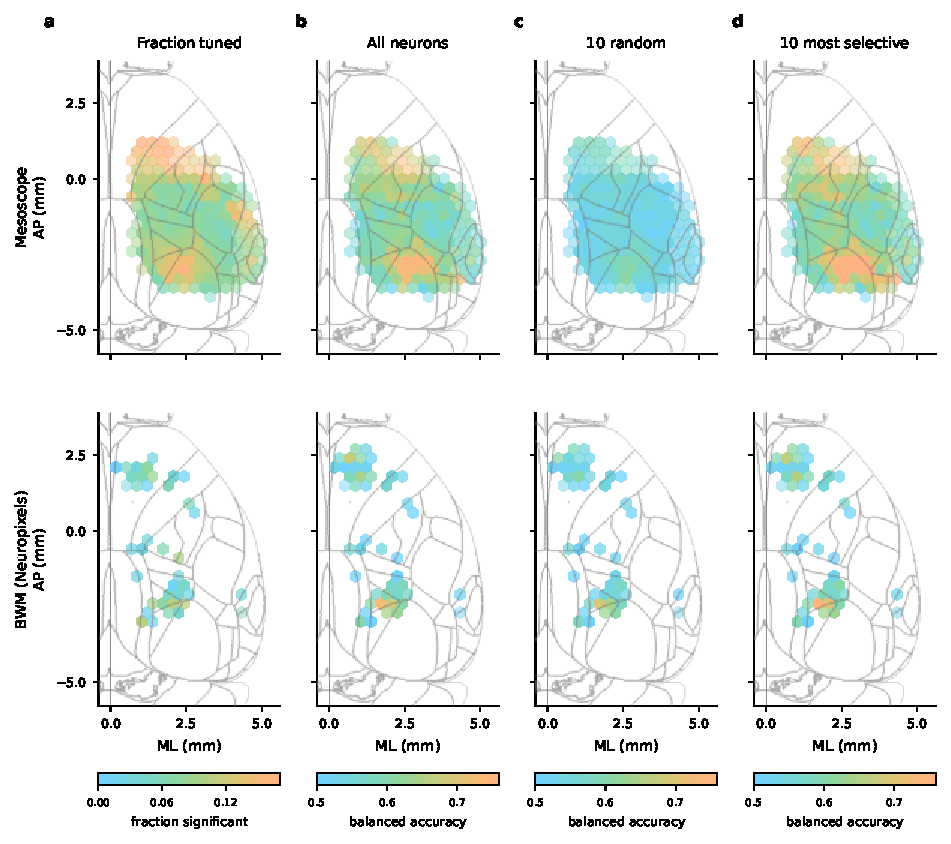
\includegraphics[width=7.00in,height=0.78\textheight,keepaspectratio]{si/si_high_contrast_panels.pdf}
  \caption{Strict inclusion: only bins (0.4\,mm vertex to vertex, hemispheres folded) with $\geq$3 sessions from $\geq$2 animals, each session contributing $\geq$10 neurons. Isoluminant colour map; opacity encodes the number of animals (2: 50\,\%, 3: 75\,\%, $\geq$4: 100\,\%), so bins backed by few animals fade towards white. Mesoscope top row, BWM bottom row. Stimulus side using only trials with contrast $\geq$25\,\% (the two highest contrasts, about 40\,\% of trials); 0\,\% and low-contrast stimuli are unlikely to drive visual cortex. Fraction of neurons tuned in visual areas (VIS*) vs elsewhere: mesoscope 0.141 vs 0.154 with all contrasts, 0.102 vs 0.106 with high contrasts; BWM 0.086 vs 0.064 and 0.051 vs 0.048 (with 40\,\% of the trials the test has less power). Decoding from all neurons of a session in visual bins (most neurons VIS*) vs other bins: mesoscope 0.589 vs 0.578 with all contrasts, 0.650 vs 0.617 with high contrasts; BWM 0.566 vs 0.532 and 0.615 vs 0.537. \textbf{a} Fraction of neurons tuned to stimulus side, tested on high-contrast trials only. \textbf{b} Stimulus side decoded from all neurons of the session in the bin, high-contrast trials only. \textbf{c} Same from 10 randomly drawn neurons (mean of 3 draws). \textbf{d} Same from the 10 most selective neurons (selected within the training folds).}
  \label{fig:si_high_contrast}
\end{figure}
